\documentclass{article}

\usepackage{float,algorithm,graphicx,hyperref}
\usepackage[noend]{algpseudocode}

\title{Lab 2 - Perceptron Algorithm}
\author{Kyle Swanson}
\date{January 9, 2018}

\setcounter{section}{-1}

\begin{document}

\maketitle

\section{Introduction}

The goal of this project is to design a linear classifier to analyze the sentiment of product reviews. The training set consists of reviews written by Amazon customers for various food products. The reviews were originally on a 5 star scale but have been adjusted to $+1$ or $-1$, representing a positive or a negative review, respectively. Table \ref{reviews} below shows an example of two reviews from the dataset and their corresponding labels.

\begin{table}[H]
    \begin{center}
        \begin{tabular}{ p{100mm} p{15mm} }
            \hline
            Review & Label \\
            \hline
            \textit{Nasty No flavor. The candy is just red , No flavor . Just plan and chewy . I would never buy them again} & $-1$ \\
            \hline
            \textit{YUMMY! You would never guess that they’re sugar-free and it’s so great that you can eat them pretty much guilt free! i was so impressed that i’ve ordered some for myself (w dark chocolate) to take to the office. These are just EXCELLENT!} & $+1$ \\
            \hline
        \end{tabular}
        \caption{Example entries from the reviews dataset. The two reviews were written by different customers describing their experience with a sugar-free candy.}
        \label{reviews}
    \end{center}
\end{table}

\noindent
In order to automatically analyze reviews, you will complete the following tasks:

\begin{enumerate}
    \item Implement a variant of the perceptron algorithm called \textit{average perceptron}.
    \item Run your classifier on the food review dataset using simple text features.
    \item Tune your model and experiment with additional features.
    \item Test your model.
\end{enumerate}

\subsection{Code}

The code for this lab is now available in the directory \texttt{Lab2} in the \texttt{IntroML} repo. In the \texttt{Lab2} directory you will find three files:

\begin{enumerate}
    \item \texttt{utils.py} - This file contains utility functions which will be called by the other files. You do not need to modify this file.
    \item \texttt{lab2.py} - Most of the project involves implementing functions specified in this file.
    \item \texttt{main.py} - Once you have implemented the relevant functions in \texttt{lab2.py}, you will uncomment the corresponding section of \texttt{main.py} and you can run the code with \texttt{python main.py}.
\end{enumerate}

\section{Perceptron Algorithm}

The first step is to implement the perceptron algorithm, which we will use to learn a classifier for food reviews. As a reminder, below is the perceptron algorithm:

\begin{algorithm}[H]
    \caption{Perceptron Algorithm}
    \label{perceptron}
    
    \begin{algorithmic}[1]
        \Procedure{Perceptron}{}
        \State $\theta = \vec{0}$ (vector)
        \State $\theta_0 = 0$ (scalar)
        \For{$t = 1, \dots, T$}
            \For{$i = 1, \dots, n$}
                \If{$y^{(i)} (\theta \cdot x^{(i)} + \theta_0) \leq 0$}
                    \State $\theta = \theta + y^{(i)} x^{(i)}$
                    \State $\theta_0 = \theta_0 + y^{(i)}$
                \EndIf
            \EndFor
        \EndFor
        \State \Return{$\theta, \theta_0$}
        \EndProcedure
    \end{algorithmic}
\end{algorithm}

\subsection{Average Perceptron}

However, rather than implementing the perceptron algorithm as is, we will implement a slight variant called \textit{average perceptron}. The classifier learned by the regular perceptron algorithm is most strongly influenced by the training examples that appear last and can be thrown off by outliers. Average perceptron aims to fix that by returning the average of $\theta$ and $\theta_0$ across all iterations rather than just returning the last $\theta$ and $\theta_0$. More precisely, the classifier returned is $\theta_{final}, {\theta_0}_{final}$ where

$$\theta_{final} = \frac{1}{nT} \left( \theta^{(1)} + \theta^{(2)} + \dots + \theta^{(nT)} \right)$$

$${\theta_0}_{final} = \frac{1}{nT} \left( \theta_0^{(1)} + \theta_0^{(2)} + \dots + \theta_0^{(nT)} \right)$$

This is most easily done by keeping track of the sum of $\theta$ and the sum of $\theta_0$ on \textit{all} iterations (not just on iterations where a mistake is made) and then dividing by $nT$, the total number of iterations.

\subsection{Implementation}

Here are the steps you need to complete in \texttt{lab2.py}:

\begin{enumerate}
\item Implement \texttt{perceptron\_single\_step\_update}, which updates the values of $\theta$ and $\theta_0$.
\item Implement \texttt{perceptron}, which runs the average perceptron algorithm. You should make use of \texttt{perceptron\_single\_step\_update} to compute the new $\theta$ and $\theta_0$ whenever the perceptron makes a mistake.
\end{enumerate}

\subsection{Results}

When you are done with your implementation, go into \texttt{main.py}, uncomment the Part 1 code, and run \texttt{python main.py}. This will run your implementation of the perceptron algorithm on a toy dataset of 2-dimensional points. If your implementation is correct, you should see the points plotted along with a reasonable-looking decision boundary.

\subsubsection{Remark}

The basic perceptron algorithm produces a decision boundary like this:

\noindent
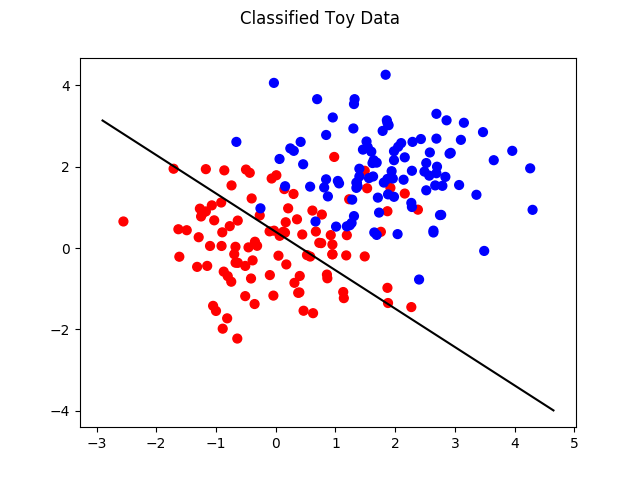
\includegraphics[width=\textwidth]{perceptron.png}

Note how this boundary is skewed towards the red points and misclassifies almost half the red points. The boundary produced by your average perceptron should be closer to the middle between the red and blue points, thereby producing a better classification.

\section{Classifying Reviews}

Now that we have a functioning perceptron classifier, we're going to use our classifier to classify Amazon food reviews.

\subsection{Data}

The data consists of reviews which have been labeled with $+1$ or $-1$, corresponding to a positive or a negative review. The data is located in the \texttt{Data} directory and has been split into three sets:

\begin{enumerate}
    \item \texttt{reviews\_train.csv} - 1800 examples
    \item \texttt{reviews\_validation.csv} - 350 examples
    \item \texttt{reviews\_test.csv} - 350 examples
\end{enumerate}

You can open the files with a text editor to get a sense of how the data looks.

We will be training our classifier on the training set of 1800 examples. To test how well the classifier generalizes to examples it hasn't seen before, we will then test our classifier on the validation set. Since the algorithm includes hyperparameters (ex. the value of $T$) which aren't directly learned, we select hyperparameters by choosing the ones which perform best on the validation set. Finally, once all hyperparameters have been determined, we test the model on the test set, which consists of examples which have not been seen in either training or validation.

\subsection{Features}

Since we can't run the perceptron directly on raw text, we need to instead extract features from the text. We will be using a \textit{bag of words} approach. We start by compiling all the words which appear in the training set into a \textit{dictionary}. Let's say the size of the dictionary is $D$. Then we can transform each review into a feature vector of length $D$ where the $i^{th}$ coordinate is $1$ if the $i^{th}$ word in the dictionary appears in the review and is $0$ otherwise. For instance, consider two simple documents: ``Mary loves apples" and ``Red apples". In this case, the dictionary is the set $\{ Mary,\ loves,\ apples,\ red\}$ and the documents are represented as $(1, 1, 1, 0)$ and $(0, 0, 1, 1)$.

\texttt{lab2.py} already includes a function, \texttt{bag\_of\_words}, which creates a dictionary, and a function, \texttt{extract\_bow\_feature\_vectors}, which uses the dictionary to create a bag of words feature vector for each review. You do not need to modify these functions, but take a look if you're curious how they work (you may want to modify them later in the lab).

\subsection{Implementation}

Your job in this section of the lab will be to write functions which take a trained $\theta$ and $\theta_0$ and use these parameters to classify reviews and then assess the accuracy of those classifications. Specifically, you will implement the following functions in \texttt{lab2.py}:

\begin{enumerate}
    \item \texttt{classify} - Takes in a feature matrix, $\theta$, and $\theta_0$. Uses $\theta$ and $\theta_0$ to classify each row (feature vector) of the feature matrix and returns a list of the classifications.
    \item \texttt{accuracy} - Takes in a feature matrix, an array of correct labels, $\theta$, and $\theta_0$. This function should first use \texttt{classify} to classify the reviews in the feature matrix and then it should compute the accuracy by comparing the classifications produced by the model to the correct labels. You can either compute the accuracy directly or use an external function such as scikit-learn's \texttt{accuracy\_score} (\url{http://scikit-learn.org/stable/modules/generated/sklearn.metrics.accuracy_score.html}).
\end{enumerate}

\subsection{Results}

After completing your implementation, uncomment Part 2 of the code in \texttt{main.py} and run \texttt{python main.py} (you may recomment the Part 1 code). If your implementation is correct, you should see two lines printed to your terminal, one with training accuracy and one with validation accuracy. Your training accuracy should be close to $1$ while your validation accuracy should be close to $0.9$.

Note that the model does much better when tested on training examples since it has seen those examples already. This is a case of mild overfitting. However, the model is still able to do well on the validation set, so it is still able to generalize.

\section{Improving the Model}

Now that we have a reasonable model, the obvious next question is: How can we make it better? In this section we will explore two methods for improving models: optimizing the hyperparameters and improving the features. We will also explore a simple method for understanding how the model makes its decisions.

\subsection{Tuning the Hyperparameters}

Hyperparameters are any model parameters which are not directly learned by the model. In the case of the perceptron algorithm, the only hyperparameter is the value of $T$, which tells the perceptron how many times to train on all of the training examples.

A common method for optimizing hyperparameters is called \textit{grid search}, which essentially just tries various combinations of hyperparameter values and chooses the set of hyperparameters which produces the best result on the validation set. Since we only have one hyperparameter, we will simply try several values of $T$ and choose the value which produces the best validation accuracy.

\subsubsection{Implementation}

Your task is to implement the function \texttt{tune}. This function should take in a list of $T$ values to try along with training features and labels and validation features and labels. For each value of $T$, it should call \texttt{perceptron} with the train features and labels and the $T$ value to train a perceptron and output a $\theta$ and $\theta_0$. Then it should use \texttt{accuracy} to determine the accuracy on the training set and on the validation set. These accuracies should be appended to a list of training accuracies and a list of validation accuracies, and the two lists should be returned as numpy arrays.

\subsubsection{Results}

Once your implementation is complete, uncomment Part 3.1 and run \texttt{main.py}. You should see a plot of train and validation accuracies for different $T$ values. Feel free to try more values of $T$ than just the ones provided. Once you have determined the $T$ value that maximizes the validation accuracy, go to \texttt{main.py} and set \texttt{T\_best} equal to that value. This value will be used for the rest of the lab.

\subsection{Understanding the Model}

An important element of machine learning is understanding how the model works, as this can often help inform your choice of model or features. Since we are using bag of words features, each coordinate of $\theta$ corresponds to a single word. Therefore, the coordinates of $\theta$ with the largest values correspond to the most important words since these words will have the greatest influence on the final value of $\theta \cdot x^{(i)}$ and will thus most influence the final classification.

In this section you do not need to write any code. A function called \\ \texttt{most\_explanatory\_words} has been implemented for you in \texttt{utils.py}. This function sorts the words by order of importance based on the values of the coordinates of $\theta$. Simply uncomment Part 3.2 in \texttt{main.py}, run the file, and observe the results. The top 10 most explanatory words will be printed to the terminal, and they should mostly match your intuition.

\subsection{Adding Features}

Perhaps the best method for improving a model like the perceptron algorithm is to select better and/or more features. The bag of words features are a great start, but they leave out important information such as word order. In this section, you are free to explore additional features in order to determine which features contribute to the best model.

\subsubsection{Implementation}

Your task is to implement \texttt{extract\_final\_features}. This function currently returns the bag of words features. You may modify this function however you see fit, as long as it returns a feature matrix with $n$ rows, one for each review. You may even modify the parameters of the function if you see fit, though it should always take in the reviews so that features can be extracted from the reviews. You may also modify the data loading section at the top of \texttt{main.py} if necessary when constructing \texttt{train\_final\_features}, \texttt{val\_final\_features}, and \texttt{test\_final\_features}. These are the features which will be used in the end to evaluate your model.

Suggestions include, but are not limited to:

\begin{enumerate}
\item Adding bag of \textit{bigram} features. These are very similar to the bag of words (also know as bag of unigrams) features, but use pairs of adjacent words rather than individual words. For instance, the documents ``Mary loves apples" and ``Red apples" would produce a bigram dictionary $\{Mary\ loves,\ loves\ apples,\ Red\ apples\}$ and the feature vectors for the two documents would be $(1, 1, 0)$ and $(0, 0, 1)$, respectively.

\item Removing \textit{stopwords}. Stopwords are common words such as ``he", ``she", ``it", ``the" which have little affect on sentiment. A list of stopwords is provided in the \texttt{Data} directory in the file \texttt{stopwords.txt}.

\item Including the length of the review (number of words) as a feature. Since the bag of words features are all either $0$ or $1$ while the length could be $100$ or more, you may want to normalize the length (i.e. divide my the maximum length) so that this feature is at roughly the same scale as the other features and won't dominate.

\item Including a feature for words in all-caps such as ``AMAZING" or ``DON'T BUY THIS".

\item Using word embeddings rather than bag of words (this is more advanced and might take some time to implement).

\item Removing uncommon words, e.g. words that appear less than three times across the training set. This reduces the number of features and thus the dimensionality of the feature vectors and $\theta$ which can help prevent overfitting.
\end{enumerate}

\subsubsection{Results}

When testing your new features, uncomment Part 3.3 of \texttt{main.py} and run the file. You will see the bag of words training and validation accuracies followed by the training and validation accuracies using your custom features. These will initially be identical because the default for the custom features is to use the bag of words features. Your goal is to maximize the validation accuracy using your custom features.

\section{Testing the Model}

Now that your model and features have been optimized on the validation set, the final step is to test the model on the test set. Uncomment Part 4 in \texttt{main.py} and run the file. Send me your training, validation, and test accuracies when you are done. The group with the best test accuracy wins. Good luck!

\end{document}
